


\begin{frame}{Multigrid}

 \begin{minipage}{0.6\textwidth}
 \begin{block}{Ingredients of Algebraic Multigrid}
  \begin{itemize}
   \item Smoother (Relaxation schemes, etc.)
   \item Coarsening
   \item Interpolation (Inter-grid transfer)
  \end{itemize}
 \end{block}
 \end{minipage}

 \begin{minipage}{0.48\textwidth}
  \begin{center}
  \includegraphics[width=0.99\textwidth]{figures/graph-rs.pdf} \\
    Classical coarsening
  \end{center}
 \end{minipage}
 \begin{minipage}{0.48\textwidth}
  \begin{center}
    \includegraphics[width=0.99\textwidth]{figures/graph-ag.pdf} \\
    Aggregation coarsening
  \end{center}
 \end{minipage}
 \vspace*{.5cm}
\end{frame}



%%%%%%%%


\begin{frame}{Multigrid Parallelization}

 \begin{block}{Setup Phase}
  \begin{itemize}
   \item Determination of coarse points in parallel by graph splitting
   \item Compute coarse operators $A^{k+1} = R^k A^k P^k$ (where $A^0 = A$)
   \item Datastructures: analyze and allocate
   \item Limited fine-grained parallelism
  \end{itemize}
 \end{block}

 %\pause
 \begin{minipage}{0.58\textwidth}
 \begin{block}{Cycle Phase}
  \begin{itemize}
   \item Parallel Jacobi Smoother
   \item Restriction $R^k x^k$, prolongation $P^k x^{k+1}$
   \item Direct solution on coarsest level
   \item Static datastructures
   \item Enough fine-grained parallelism
  \end{itemize}
 \end{block}
 \end{minipage}
 \begin{minipage}{0.4\textwidth} \vspace*{-1.5cm}
  \includegraphics[width=0.99\textwidth]{figures/graph-rs0.pdf} \\ \vspace*{0.1cm}
  \includegraphics[width=0.99\textwidth]{figures/multigrid-cycles.png}
 \end{minipage}

 \vspace*{0.5cm}

\end{frame}


%%%%%%%%%%

\begin{frame}{AMG Sparse Matrix-Matrix Multiplication}
 \begin{block}{Coarse Grid Operator}
  \begin{itemize}
   \item $A^{\mathrm{coarse}} = R A^{\mathrm{fine}} P$
   \item Common choice: $R = P^{\mathrm{T}}$
  \end{itemize}
 \end{block}

 \begin{block}{Computation}
  \begin{itemize}
   \item Explicitly set up $R = P^{\mathrm{T}}$ (hard in parallel)
   \item $C = A^{\mathrm{fine}} P$
   \item $A^{\mathrm{coarse}} = R C$
  \end{itemize}
 \end{block}

\end{frame}


\begin{frame}{AMG Sparse Matrix-Matrix Multiplication}
  \begin{center}
    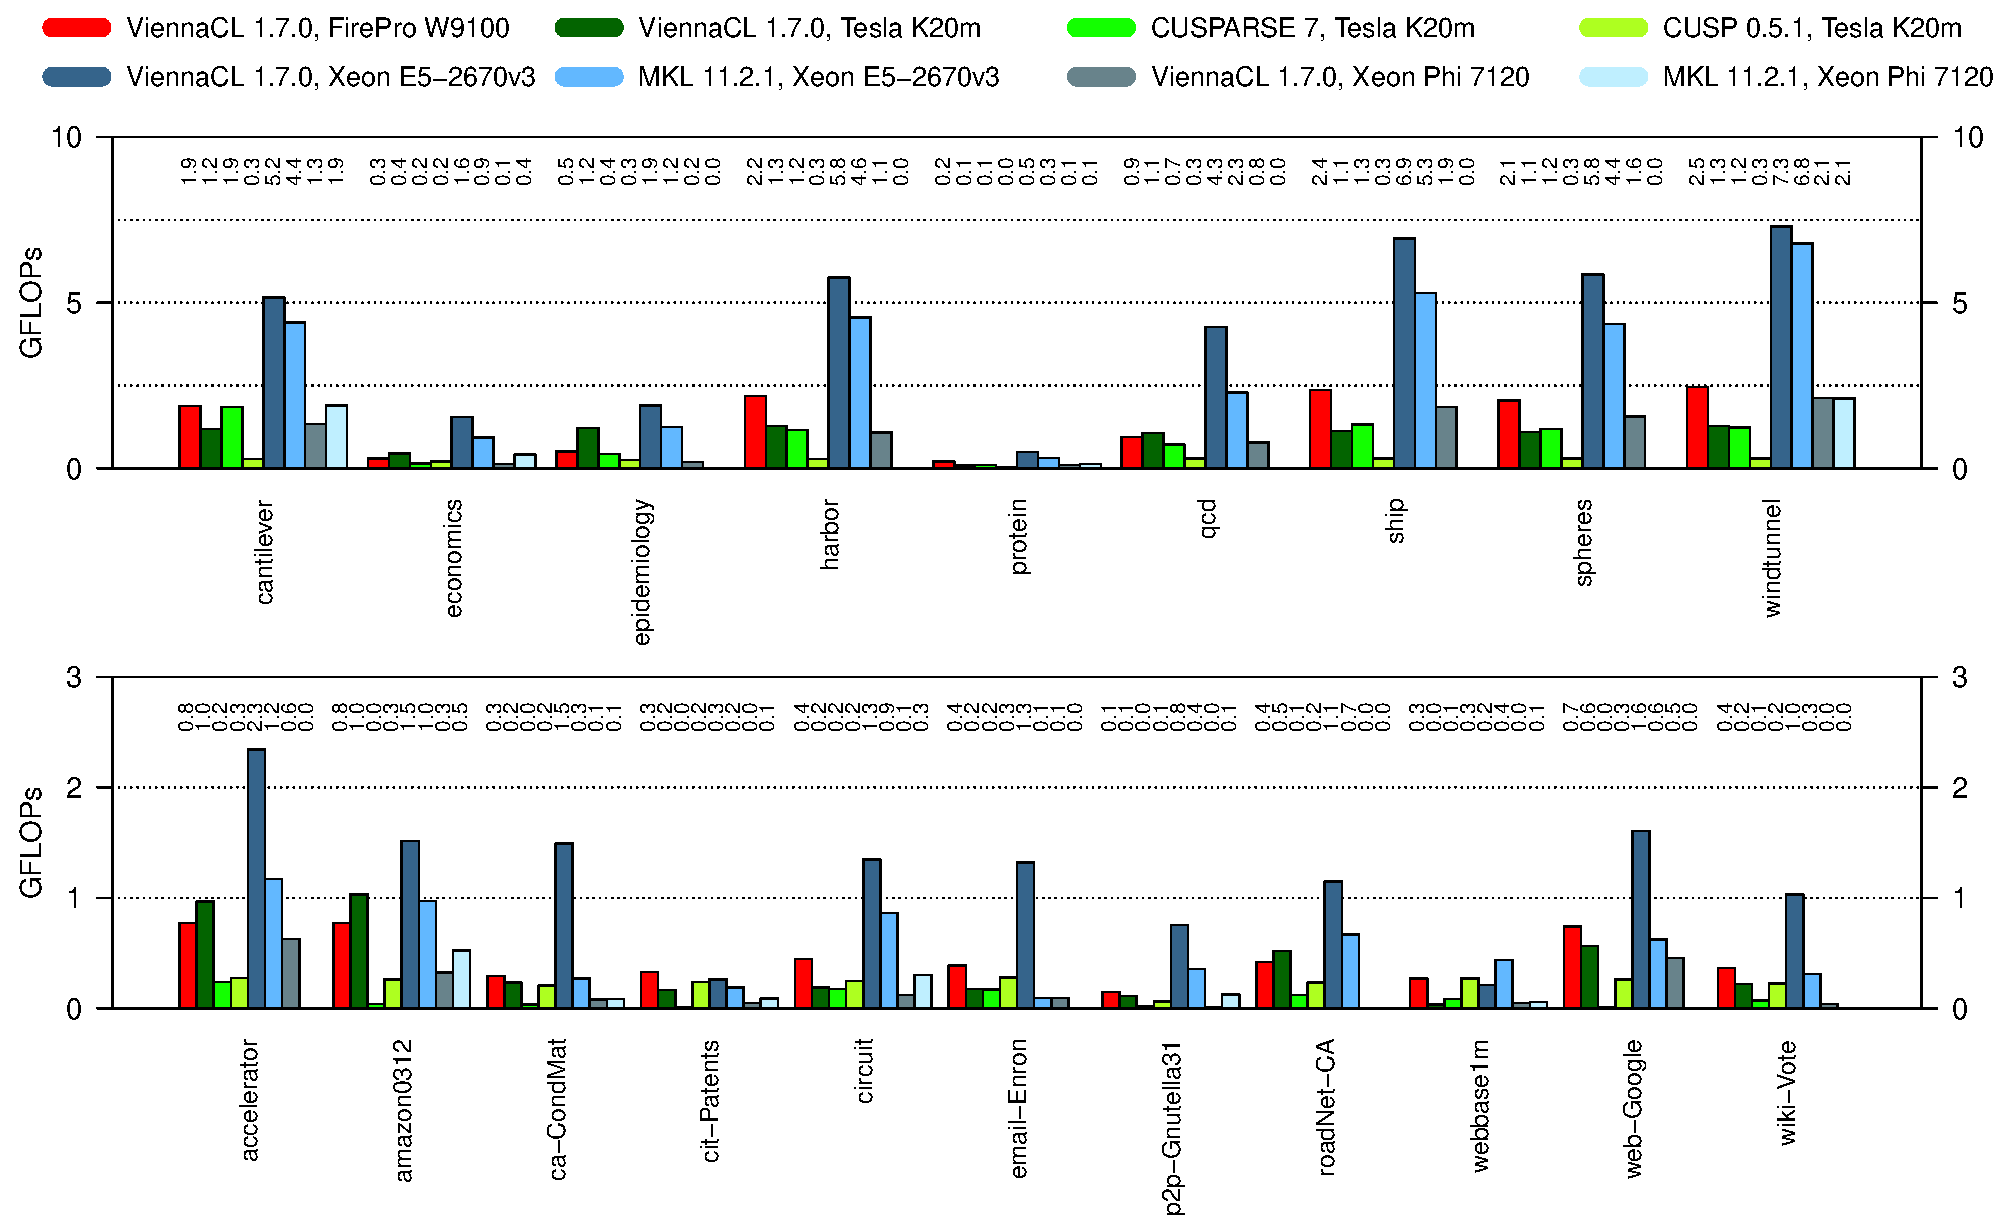
\includegraphics[width=0.95\textwidth]{spgemm}
  \end{center}
\end{frame}


%%%%%%%%%%%%


\begin{frame}{AMG Benchmark}
  \begin{center}
    \includegraphics[width=0.95\textwidth]{amg-vs-pure-full-2d-4}
  \end{center}
\end{frame}
